% Appendix Template

\chapter{Two-photon Imaging Using Chaotic Sources} % Main appendix title

\label{AppendixThermal} % Change X to a consecutive letter; for referencing this appendix elsewhere, use \ref{AppendixX}

%\subsubsection{Two-photon Imaging Using Chaotic Sources}

In principle the term "thermal radiation" should refer only to radiation coming 
from a blackbody in thermal equilibrium at some temperature T. But with this realisation of thermal radiation
we have to face some characteristics of true thermal fields. Thermal radiation is also referred as chaotic light, 
which have extreme short coherence time. This is because a thermal source contains a large number of independent sub-sources,
such as the trillions of atoms or molecules.These atomic transitions that can be identical or different
act like sub-sources, that emit light into independently and randomly. 



\begin{figure}[h!]
\centering
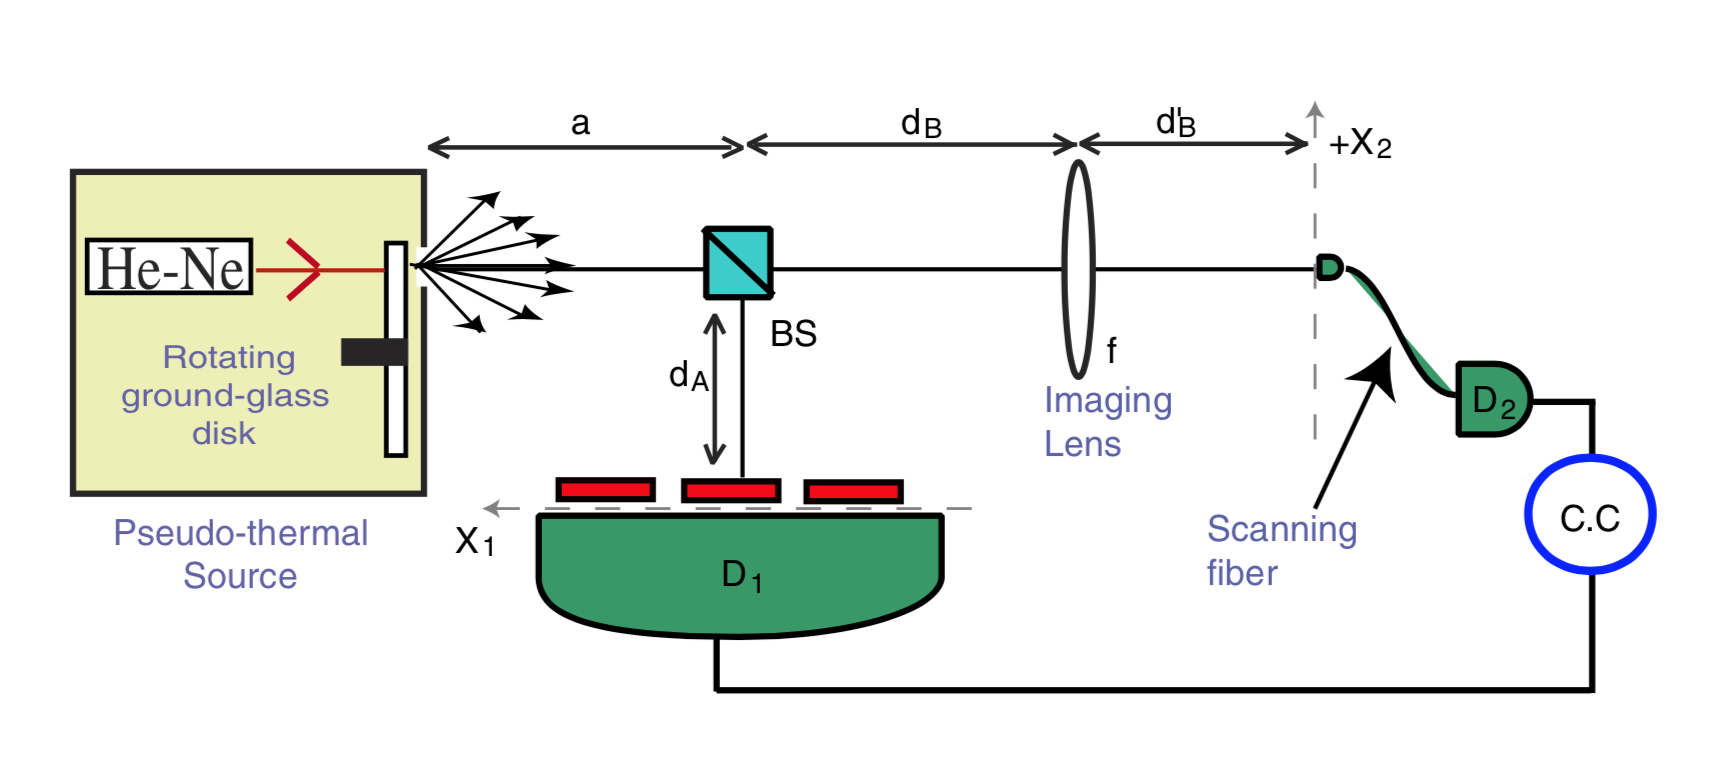
\includegraphics[width=0.6\textwidth]{Figures/thermalSetup.png}
\caption{Experimental setup for the Two-photon imaging using thermal light, taken from \cite{thermalAlejandra}} 
\label{fig:thermalSetup}
\end{figure}
The source light in Figure \ref{fig:thermalSetup} is the one developed by Martinssen and Spiller\cite{intensity}
which is the most commonly used among the pseudothermal fields. A  coherent laser radiation is focused on a rotating ground glass disk, 
the scattered radiation is chaotic with a Gaussian spectrum. After this, a nonpolarizing beam
splitter (BS) splits the radiation in two distinct optical pths, In the reflected arm an object, with 
transmission function $T(r_1)$, is placed ar a distance $d_A$ from the BSand a bucket detector ($D_1$)
is just behind the object. In the transmitted arm an imaging lens, with focal lenght $f$, is placed at a 
distance $d_B$ from the BS, and a multimode optical fiber ($D_2$) scans the transverse plane
at a distance $d'_B$ from the lens. The output pulses from the two single photon counters are sent 
to an electronic coincidence circuit to measure the rate of coincidence counts.

Once again we expect the joint-detection counting rate between photodetectors $D_1$ and $D_2$ to behave
like the one described in Eq. \ref{eq:coincidences}. But thos rate this coincidence counts is governed
by the second-order Glauber correlation function \cite{glauber}:
\begin{equation}
G^{(2)} (\vec{r}_1; \vec{r}_2) \equiv \langle E^{(-)}_1(\vec{r}_1)E^{(-)}_2(\vec{r}_2) \times E^{(+)}_2(\vec{r}_2)E^{(+)}_1(\vec{r}_1) \rangle
\end{equation}
where the $E^{(-)}$ and $E^{(+)}$ are the negative-frequency and the positive-frequency field operators describing the detection events at the
locations $\vec{r}_1$ and $\vec{r}_2$. The transverse second-order correlation correlation function 
for a thermal source is given by \cite{thermalAlejandra}:
\begin{equation}\label{eq:thermal}
G^{(2)}_{\textit{thermal}}(\vec{r}_1; \vec{r}_2) \propto \sum_{\vec{q}} |g_1(\vec{q},\vec{r}_1)|^2
\sum_{\vec{q}'} |g_2(\vec{q}',\vec{r}_2)|^2 + |\sum_{\vec{q}} g_1^*(\vec{q},\vec{r}_1) g_2(\vec{q},\vec{r}_2)|^2
\end{equation}
where $\vec{r}_i$ is the transverse position of the detector $D_i$, $\vec{q}$ and $\vec{q}'$
are the transverse components of the momentum vectors, and $g_i(\vec{q},\vec{r}_i)$ is the Green's function 
associated with the propagations of the field with transverse momentum $\vec{q}$ from the source, 
to the position $\vec{r}_i$ at the detection plane defined by the detector $D_i$. $g_i(\vec{q},\vec{r}_i)$ is defined in a similar way 
as in Eq. \ref{eq:green}.

It is important to note that there are two main differences with respect to the SPDC case: 
First the presence of a background noise (first term of Eq. \ref{eq:thermal}), which does not exist for SPDC. Second,
the possibility of writing the second term of Eq. \ref{eq:thermal} as a product of the first order correlation
functions, $G^{(1)}_{12}G^{(1)}_{21}$, while there is no way to write the biphoton produced by the 
SPDC as a product of other correlations. Also this term $|\sum_{\vec{q}} g_1^*(\vec{q},\vec{r}_1) g_2(\vec{q},\vec{r}_2)|^2$
Is the interference of intensities of a incoherent statistical assemble of randomly distributed photons.


Following the proces done in \cite{thermalAlejandra}, it can be shown that for any values of distances
$d_A$, $d_B$ and $d_{B}'$ which obey the equation:
\begin{equation}
\frac{1}{d_B - d_A} + \frac{1}{d_{B}'} = \frac{1}{f}
\end{equation}
which clearly has the form on a thin-lens equation, defining a point-to-point correspondence between imaging and object plane.
Then Eq. \ref{eq:thermal} can be simplified as:
\begin{equation}
G^{(2)}_{\textit{tot}}(\vec{r}_2) \propto N + | T \left( \frac{d_A - d_B}{d_{B}'} \vec{r}_2 \right) |^2
\end{equation}
where $T ( \frac{d_A - d_B}{d_{B}'} \vec{r}_2 )$ is the object transmission function ($T(\vec{r}_1)$)
reproduced on the $D_2$ plane. Thanks to this result we can conclude that a thermal source allows reproducing
in coincidence measurements the two-photon image of an object, similarly to the SPDC case, except for a 
constant background noise, where $N$ is proportional to it.


It is possible to establish an analogy
between classical optics and entangled two-photon optics:
the two-photon probability amplitude plays in entangled
two-photon processes the same role that the complex amplitude
of the electric field plays in classical optics  \cite{thermalAlejandra}.